%\documentclass[wcp,gray]{jmlr} % test grayscale version
\documentclass[wcp]{jmlr}

% The following packages will be automatically loaded:
% amsmath, amssymb, natbib, graphicx, url, algorithm2e

%\usepackage{rotating}% for sideways figures and tables
\usepackage{longtable}% for long tables

% The booktabs package is used by this sample document
% (it provides \toprule, \midrule and \bottomrule).
% Remove the next line if you don't require it.
\usepackage{booktabs}
% The siunitx package is used by this sample document
% to align numbers in a column by their decimal point.
% Remove the next line if you don't require it.
%\usepackage[load-configurations=version-1]{siunitx} % newer version
%\usepackage{siunitx}

\usepackage{tikz}

\newcommand{\icon}[1]{\tikz[baseline=-3pt] \node[inner sep=0pt,outer sep=0pt]{\includegraphics[height=1.1em]{images/#1}};}

% The following command is just for this sample document:
\newcommand{\cs}[1]{\texttt{\char`\\#1}}

\jmlrvolume{41}
\jmlryear{2015}
\jmlrworkshop{BIGMINE 2015}

\title[Big Data with ADAMS]{Big Data with ADAMS}

 % Use \Name{Author Name} to specify the name.
 % If the surname contains spaces, enclose the surname
 % in braces, e.g. \Name{John {Smith Jones}} similarly
 % if the name has a "von" part, e.g \Name{Jane {de Winter}}.
 % If the first letter in the forenames is a diacritic
 % enclose the diacritic in braces, e.g. \Name{{\'E}louise Smith}

 % Two authors with the same address
 % \author{\Name{Author Name1} \Email{abc@sample.com}\and
 %  \Name{Author Name2} \Email{xyz@sample.com}\\
 %  \addr Address}

 % Three or more authors with the same address:
 % \author{\Name{Author Name1} \Email{an1@sample.com}\\
 %  \Name{Author Name2} \Email{an2@sample.com}\\
 %  \Name{Author Name3} \Email{an3@sample.com}\\
 %  \Name{Author Name4} \Email{an4@sample.com}\\
 %  \Name{Author Name5} \Email{an5@sample.com}\\
 %  \Name{Author Name6} \Email{an6@sample.com}\\
 %  \Name{Author Name7} \Email{an7@sample.com}\\
 %  \Name{Author Name8} \Email{an8@sample.com}\\
 %  \Name{Author Name9} \Email{an9@sample.com}\\
 %  \Name{Author Name10} \Email{an10@sample.com}\\
 %  \Name{Author Name11} \Email{an11@sample.com}\\
 %  \Name{Author Name12} \Email{an12@sample.com}\\
 %  \Name{Author Name13} \Email{an13@sample.com}\\
 %  \Name{Author Name14} \Email{an14@sample.com}\\
 %  \addr Address}


 % Authors with different addresses:
  \author{\Name{Peter Reutemann} \Email{fracpete@waikato.ac.nz} \\
  \Name{Geoff Holmes} \Email{geoff@waikato.ac.nz}\\
  \addr Department of Computer Science \\
  The University of Waikato \\
  Hamilton, NZ
 }

%\editors{List of editors' names}

\begin{document}

\maketitle

\begin{abstract}
ADAMS is a modular open-source Java framework for developing workflows available for
academic research as well as commercial applications. It integrates
data mining applications, like MOA, WEKA, MEKA and R, image and video
processing and feature generation capabilities, spreadsheet and database
access, visualizations, GIS, webservices and fast protoyping of new 
functionality using scripting languages (Groovy/Jython).
\end{abstract}
\begin{keywords}
workflow, big data, data streams, twitter, video, spectral data
\end{keywords}

\section{Introduction}
The origins of ADAMS lie in academia, with the project originally being developed to process analytical data from gas-chromatography mass-spectrometry instruments (\cite{gcms}), in order to handle many pre-processing steps and various predictions in parallel. However, the framework now forms the basis of commercial applications, as it allows for rapid development of data mining applications that integrate into business processes. The framework, written in Java and released under GPLv3
%\footnote{\url{http://www.gnu.org/licenses/gpl-3.0.txt}{}}
, consists of various modules grouped by functionality. It includes MOA (\cite{moa}), WEKA (\cite{weka}), MEKA (\cite{meka}), R, image/video processing and feature generation, spreadsheet and database handling, various visualizations, GIS support through OpenStreetMap, webservices, and scripting (Jython or Groovy) for fast prototyping.

The remainder of the paper is structured as follows: first, a quick introduction to the framework is given. Second, an overview of some of the research areas that it can be used for. Third, a commercial application that is based on the framework.

\section{Framework}
Workflow systems, like RapidMiner, KNIME or Kepler, use a canvas approach for placing operators and combining them by connecting them. On the one hand, this is a very intuitive approach, since the user can see how the data flows. On the other hand, this can make modifying the flow a tedious process, as the authors experienced: disconnecting operators, moving them around, inserting other operators, reconnecting operators and so forth. Despite birds-eye-view and meta-operators that group several operators together, the canvas approach can quickly become hard to comprehend and doesn't seem to scale well when dealing with hundreds or even thousands of operators.

\begin{figure}[htb]
  \begin{minipage}[b]{0.5\linewidth}
  \centering
  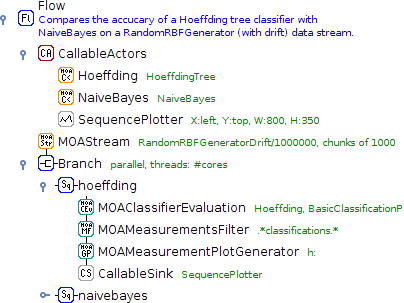
\includegraphics[width=7.0cm]{images/example_flow_clipped.png}
  \caption{Comparing two MOA classifiers.}
  \label{example_flow}
  \end{minipage}%
  \begin{minipage}[b]{0.5\linewidth}
  \centering
  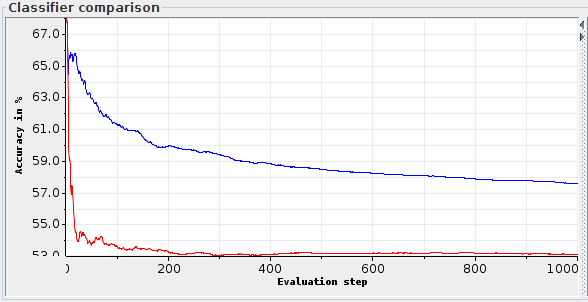
\includegraphics[width=8.0cm]{images/example_output_clipped.png}
  \caption{Comparison output.}
  \label{example_output}
  \end{minipage}
\end{figure}

For a simple streaming experiment that compares the accuracy of two classifiers (see Figure \ref{example_flow}), the following steps would be set up in a flow: a stream generator that provides the data for training the classifiers; branching the data into two separate branches, each training and evaluating a classifier; the metric under investigation, i.e., accuracy, is extracted at specified intervals and turned into a plot data point; the plotting data from both classifiers is channelled into the same plot for direct comparison (see plot in Figure \ref{example_output}).

ADAMS forfeits some of the advantages and asthetics of this canvas approach to provide a more compact layout, using a simple tree structure instead for organizing its operators, which are called actors. The nesting of nodes in the tree resembles the nesting of actors programmatically, based on whether the actor is a primitive one (e.g., filtering a dataset) or one that manages other actors (e.g., grouping actors to be executed sequentially). So-called control actors determine data flow and flow execution: a \icon{Branch} Branch actor forwards the incoming data to all of its sub-actors, i.e., the sub-branches; a \icon{Sequence}~Sequence actor executes its sub-actors one-by-one using the output of one actor as the input for the next one. The four types of combinations that result from input and output handling, are as follows: \icon{CallableActors}~Standalone, which has no input nor output, e.g., a database connection; \icon{MOAStream}~Source, which only generates output; \icon{MOAClassifierEvaluation}~Transformer, which takes input and generates output; \icon{SequencePlotter}~Sink, which only consumes data. By using data flow control actors, it is possible to get rid of explicit connections between the actors. However, a tree structure only handles 1-to-n connections. In order to simulate n-to-m semantics, several techniques are implemented: use of containers to combine multiple outputs; support for variables, to be attached to parameters of actors or simply used for calculations; internal key-value storage for storing, retrieving and updating data in multiple locations; and callable actors that can be invoked from anywhere in the flow using their name. Interoperability of actors is statically checked by comparing the types of data that a preceding actor can output and what types the following actor can handle. This type information in combination with the context induced by the tree structure, makes it possible to limit the actors that can be placed within a given context. Furthermore, context-aware rules can be specified for common sequences of actors (e.g., load dataset $\rightarrow$ set class attribute $\rightarrow$ cross-validate dataset $\rightarrow$ output results) aiding the user in creating flows more rapidly.

Adding new actors is straightforward: all it needs is a class either derived from one of the abstract superclasses or implementing the core interfaces for actors, placed in one of the packages which ADAMS inspects for actors and a little icon to be displayed in the editor.

\section{Research}
Given its origins, ADAMS is well-positioned for research. One of the standalone tools for stream analysis is MOA, which offers a user interface for running experiments, evaluating algorithms and visualizing metrics. However, in a workflow context, stream analysis becomes much more interesting, as filters can be appplied to the stream, compare several algorithms in parallel and plot their performance in a single plot (see Figures \ref{example_flow} and \ref{example_output}). Classification and regression experiments, as well as cluster visualizations are possible (see Figure \ref{cluster_visualization}).

Another area of research is Tweet analysis: tweets can be recorded and their associated meta-data using the public Twitter API, storing them for future replay. This tweet stream replay functionality allows the same experiment to be performed as often as required, using the same stream of tweets each time, applying different filters (e.g., checking for meta-data) and/or algorithms. Tweets with geotagging information can be displayed using the OpenStreetMap GIS functionality, allowing for visualization of geographical phenomena.

Due to a recently started collaboration with the Biology department, processing videos has been added to ADAMS. Videos get processed in near real-time, with frames being obtained at specific intervals. Apart from tracking objects, in our case tracking mice and rats during behavioural experiments (see Figure \ref{object_tracking_mouse}), it is also possible to use the image processing and feature generation functionality to generate input for machine learning algorithms, like MOA or WEKA.

\begin{figure}[htb]
  \begin{minipage}[b]{0.5\linewidth}
  \centering
  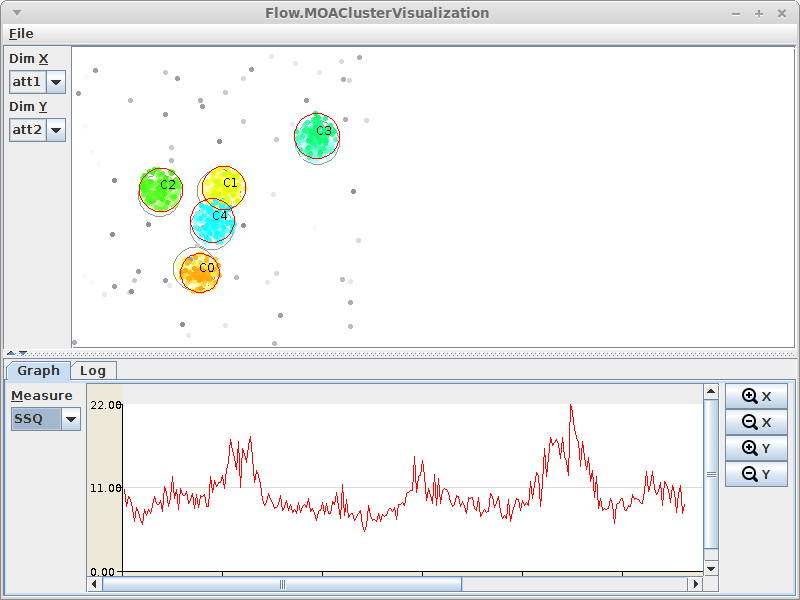
\includegraphics[width=6.5cm]{images/cluster_visualization.png}
  \caption{MOA cluster visualization.}
  \label{cluster_visualization}
  \end{minipage}%
  \begin{minipage}[b]{0.5\linewidth}
  \centering
  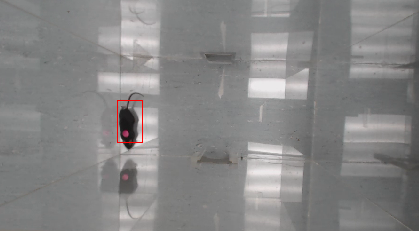
\includegraphics[width=8.0cm]{images/object_tracking_mouse.png}
  \caption{Tracking mice movements.}
  \label{object_tracking_mouse}
  \end{minipage}
\end{figure}


\section{Industry}
A commercial application based on the ADAMS framework is used for spectral analysis, encompassing near-infrared (NIR), mid-infrared (MIR) and X-ray fluorescence (XRF). One of our customers, BLGG AgroXpertus
%\footnote{\url{http://blgg.agroxpertus.nl/}{}}
, is a large environmental laboratory in Europe with multiple sites across Europe. Traditionally, they analyzed plant and soil samples using only wet chemistry. This is a lengthy and costly process that can take up to a week and  includes sample preparation, with toxic by-products, and the chemical analysis to determine concentrations of various compounds. However, when analyzing the samples in tandem with a rapid spectral technique, it is possible to build regression models with very good correlation and small errors. The number of data points per raw spectrum depends on the method and instrument, but is roughly 10,000 for XRF, 2,000 for MIR and 1,500 for NIR. The largest model for NIR is for soil and encompasses about 150,000 spectra. Altogether, BLGG uses around 250 different models for predicting various plant and soil properties. During normal operation, roughly 1,000 samples are processed each day, but during soil season (per legislation, every farmer in the Netherlands has to send in samples every four years) this goes up to 2-3,000 per day. By predicting the various concentrations using a rapid analysis technique like NIR, the number of samples that need to get analyzed via wet chemistry can be reduced significantly. The system has been in place now since 2006 and saves the company, at the time of writing, US\$ 18 million per annum and US\$ 33 million per annum during soil season. Using spectral analysis also enabled BLGG to scale up their operations. The use of machine learning here is a good repsonse to Kiri Wagstaff's \textit{Impact Challenge \#2: ``\$100M saved through improved decision making provided by an ML system''}, that she posed in 2012 for \textit{machine learning that matters} (\cite{wagstaff}).

One difference to the default ADAMS framework is that this system uses a meta-flow approach. With these meta-flows, the customer only defines certain properties of a model, e.g., data cleaning, modelling parameters and evaluation, but not any of the low-level steps. Workflow generators then take these settings and turn them, on the fly, into actual worker flows (with thousands of actors) performing all the required data collection, processing and predictions steps for the different models.

\acks{The authors would like to thank the organizers, especially Albert Bifet, for inviting us to present our work.}

\bibliography{bigmine15-adams-paper}

\end{document}
